A wide variety of physical phenomena are modeled in the space-time domain by partial differential equations. The purpose of this section is to review generalities about PDEs and suited strategies depending on the natures of equations so that solutions can be derived.
\subsection{General concepts}
A system of partial differential equations can be written by means of a vector operator $\vect{\Gc}$ of independent and dependent variables $(x_1,...,x_N)$ and $(u_1,...,u_I)$:
\begin{equation}
  \label{eq:diff_operator}
  \vect{\Gc}\(x_1,...,x_N,u_1,...,u_I,\drond{u_1}{x_1},..., \drond{^Mu_I}{x_N^M}\) = \vect{0}
\end{equation}
The dimension of the system is given by the size $I$ of the array $\vect{\Uc}^T=[u_1,...,u_I] \in \Rbb^I$, referred to as the \textit{unknown vector}. The highest derivative of the unknown vector in the system defines the \textit{order of the system} $N$. In equation \eqref{eq:diff_operator} and in what follows, sans-serif symbols refer to matrices while calligraphic symbols stand for column arrays. Furthermore, the partial derivatives of a quantity $u$ with respect to a variable $x$ may be written $u_x$ when there will be no ambiguity. Making use of index notation and convention of implicit summation over repeated indices, a system of partial differential equations reads:
\begin{equation*}
  \sum_{k=1}^{N}\Asf_{ij}^p \drond{^p\Uc_j}{x_k^p} + \Sc_i = 0
\end{equation*}
or equivalently, in matrix form:
\begin{equation}
  \label{eq:diff_system_matrix}
  \sum_{k=1}^{N}\tens{\Asf}^p \drond{^p\vect{\Uc}}{x_k^p} + \vect{\Sc} =  \vect{0}
\end{equation}
Coefficients matrices $\tens{\Asf}^p$ and the vector $\vect{\Sc}$ may depend on independent variables and the unknown vector ($x_1,...,x_N,\vect{\Uc}$) leading to different types of partial differential systems. Namely, whether those terms are functions of the $x_k$ are not leads respectively to \textit{linear systems with variable coefficients} or to \textit{linear systems with constant coefficients}. The system remains \textit{linear} if $\vect{\Sc}$ depends linearly on $\vect{\Uc}$, and is \textit{semi-linear} if the relation is non-linear. Finally, if the $\tens{\Asf}^p$ depend on independent variables $\vect{\Uc}$ and its derivatives up to order $M-1$, the system is called \textit{quasi-linear}.


The \textit{Initial Value Problem (IVP)} or \textit{Cauchy problem} consists in finding a solution $\vect{\Uc}$ of system \eqref{eq:diff_system_matrix} that satisfies a set of given initial conditions. Geometrically speaking, the solution of such a problem can be seen as the building of a hyper-surface surface of $\Rbb^{I+N}$, hence the term of \textit{integral surface} for $\vect{\Uc}$. Such a problem can be reduced to that of solving a first order IVP by using suitable changes of variables \cite[p.54]{PDEs}, we will therefore focus on first order PDEs.

\subsection{Notion of characteristics -- Hyperbolic problems}
The theorem of \textit{Cauchy--Kowalewski} locally ensures the existence of solutions of a Cauchy problem for partial differential systems and is based on the restrictive requirement of analytic coefficients matrices and initial data (see \cite[p.46]{PDEs}). The case of first order systems however, only requires continuity and differentiability conditions and lies on the concept of \textit{characteristics}, which makes the development of a solution more flexible.

\subsubsection*{First order quasi-linear equations}
To illustrate the aforementioned notions, we consider the first order quasi-linear PDE with independent variables $x$ and $t$:
\begin{equation}
  \label{eq:1st_order_pde}
   a u_x + b u_t  = c
\end{equation}
where coefficients $a$ and $b$ are such that $a^2 + b^2 \neq 0$. Initial values of $u$ are prescribed along a curve $\Cscr_0:\varphi(x,t)=const$ in the $(x,t)$ plane, thus defining a curve $\Cscr$ of the space $(x,t,u)$.
Moreover, we assume that $\Cscr_0$ is regular, namely $\varphi_x^2 + \varphi_t^2 \neq 0$, and that one of the partial derivatives does not vanish, say $\varphi_\x \neq 0$.

\begin{figure}[h]
  \centering
  \begin{tikzpicture}
  \begin{axis}[view={30}{30},ticks=none,xlabel=$x$,ylabel=$t$,zlabel=$u$,zmin=0,ymax=5.2]
    \addplot3[Orange,very thick,domain=0:10,samples=60,samples y=0]
    ({x},
    {4+sin(1.5*x*x)},
    {4+3.*cos(deg(x))});
    \addplot3[Duck,dashed,very thick,domain=0:10,samples=60,samples y=0]
    ({x},{4+sin(1.5*x^2)},{0*x});
    \legend{$\Cscr$,$\Cscr_0$};
    % dt/dx = -phi_x/phi_t 
    \addplot3[thick]  coordinates {(5,4+sin(1.5*25),0) (6.5,4+sin(1.5*25),0)}  node[above] at (axis cs:6.9,4.05+0.6087-0.4,0.) {\large$\varphi_t$};
    \addplot3[thick]  coordinates {(5,4+sin(1.5*25),0) (6.5,4+sin(1.5*25)+0.3,0)};
    \addplot3[thick]  coordinates {(6.5,4+sin(1.5*25),0) (6.5,4+sin(1.5*25)+0.3,0)} node[right] at (axis cs:6.7,4.05+0.6087+0.,0.) {\large$-\varphi_x$};
  \end{axis}
\end{tikzpicture}
%%% Local Variables:
%%% mode: latex
%%% TeX-master: "../../mainManuscript"
%%% End:

  \caption{Example of initial curve $\Cscr$ of the $(x,t,u)$ space and its projection $\Cscr_0$ in the $(x,t)$ plane.}
  \label{fig:initial_curve}
\end{figure}
With initial data given along $\Cscr$, the Cauchy problem is equivalent to that of finding a surface $u(x,t)$ that contains the initial curve and satisfies \eqref{eq:1st_order_pde}. Thus, one seeks the derivatives of $u$ along the initial curve. Since $u=u(\varphi(x,t))$ along $\Cscr$, one has $u_x = u' \varphi_x $ and $u_t = u' \varphi_t$ from which one deduces:
\begin{equation*}
  u_t = \frac{\varphi_t}{\varphi_x}u_x 
\end{equation*}
This relation enables to rewrite the PDE \eqref{eq:1st_order_pde} as:
\begin{equation}
  \label{eq:normal_form_pde}
  (a + b\frac{\varphi_t}{\varphi_x})u_x = c
\end{equation}
On the other hand, the total derivative of $\varphi(x,t)=const$ being $d\varphi = \varphi_x dx + \varphi_t dt =0$, equation \eqref{eq:normal_form_pde} becomes:
\begin{equation}
  \label{eq:normal_form_pde_2}
  (a - \ddroit{x}{t}b)u_x = c
\end{equation}
Hence, the Cauchy problem admits an unique solution if and only if:
\begin{equation}
  \label{eq:non-characteristics}
  \ddroit{x}{t}\neq \frac{a}{b}
\end{equation}
A \textit{non-characteristic curves} is an initial curve satisfying the condition \eqref{eq:non-characteristics}, otherwise it is a \textit{characteristic curve}. 

\subsubsection*{Geometrical representation of characteristic curves}
Let $u(x,t)$ be a surface of the $(x,t,u)$ space with normal vector is $\vect{n}=[u_x,u_t,-1]$. This surface is an integral surface if it is a solution of equation \eqref{eq:1st_order_pde} and hence, if $\vect{n}$ is perpendicular to the vector $\vect{w}=[a,b,c]$.
The set of tangent planes of every solutions $u^{(i)}(x,t)$ of equation \eqref{eq:1st_order_pde} thus forms a fan of planes which axis is $\vect{w}$.
This defines \textit{characteristic line elements} tangent to all integral surfaces $u^{(i)}(x,t)$:
\begin{equation}
  \label{eq:monge_axis}
  \matrice{dx \\ dt \\ du} = \matrice{a \\ b \\c}
\end{equation}
Introduction of a parameter $\eta$ and integration of equation \eqref{eq:monge_axis} yields a one-parameter family of \textit{characteristic curves} of the PDE:
\begin{equation*}
  x=x(\eta) \quad ; \quad t=t(\eta) \quad ; \quad u=u(\eta)
\end{equation*}
Hence, a characteristic curve is tangent at every point to all the integral surfaces, and an infinity of integral surfaces cross one characteristic curve. As a consequence, if the initial curve is a characteristic curve, infinitely many integral surfaces contain it so that the Cauchy problem can not be solved.

However, the following statement holds \cite[Ch.1]{Courant}:
\begin{theorem}[Courant]
  \label{th:integral_surface_generated}
  Every surface $u(x,t)$ generated by a one-parameter family of characteristic curves is an integral surface. Conversely, every integral surface is generated by a one-parameter family of characteristic curves.
\end{theorem}
This theorem will be used in what follows to solve the Cauchy problem.

\subsection{The method of characteristic}
We now extend the concept of characteristic curves to first order quasi-linear systems of dimension $I$. In matrix form:
\begin{equation}
  \label{eq:1st_order_quasi-linear_syst}
  \Absf^t\(x,t,\vect{\Uc}\) \: \vect{\Uc}_t + \Absf^x\(x,t,\vect{\Uc}\)\: \vect{\Uc}_x + \vect{\Sc} = \vect{0}
\end{equation}
Similarly to quasi-linear PDEs, initial conditions of $\Ucb$ are given along a regular curve $\Cscr_0:\varphi(x,t)=const$ defining the initial curve $\Ucb(\varphi(x,t))$ of the $(x,t,\Ucb)$ space. The Cauchy problem consists in finding all the derivatives of $\Ucb(x,t)$ such that equation \eqref{eq:1st_order_quasi-linear_syst} is satisfied in the vicinity of $\Cscr$.
Noticing that along the initial curve $\Ucb_x = \Ucb' \varphi_x$ and $\Ucb_t = \Ucb' \varphi_t$, one gets:
\begin{equation*}
  \vect{\Uc}_x\varphi_t - \vect{\Uc}_t\varphi_x= \vect{0}
\end{equation*}
Hence, system \eqref{eq:1st_order_quasi-linear_syst} can be rewritten:
\begin{equation}
  \label{eq:normal_form}
  \( \Absf^x - \lambda \Absf^t \) \vect{\Uc}_x + \vect{\Sc} = \vect{0} 
\end{equation}
where:
\begin{equation}
  \label{eq:lambda_slope}
  \lambda=-\frac{\varphi_t}{\varphi_x}=\ddroit{x}{t}
\end{equation}
The Cauchy problem admits an unique solution $\vect{\Uc}_x$ along $\Cscr$ if the determinant of the system does not vanish, that is:
\begin{equation}
  \label{eq:characteristic_determinant}
  D=\abs{\Absf^x - \lambda \Absf^t} \ne 0
\end{equation}
where D is called the \textit{characteristic determinant} of system \eqref{eq:1st_order_quasi-linear_syst}. If D does not have real roots along $\Cscr_0$, the problem is said \textit{elliptic} and the Cauchy problem can be solved. Indeed, in that case the knowledge of $\Ucb$ along the initial curve allows the computation of derivatives and hence, the building of an integral strip defined by $\Ucb,\Ucb_x,\Ucb_t$. If equation \eqref{eq:1st_order_quasi-linear_syst} admits $I$ real roots on the other hand, system \eqref{eq:normal_form} can no longer be solved. Those eigenvalues come along with left and right eigenvectors respectively defined as:
\begin{equation}
  \label{eq:eigenvectors}
  \Lc^k_i  \Asf^x_{ij} = \lambda_k \Lc^k_i \Asf^t_{ij} \quad ; \quad \Asf^x_{ij}\Rc^k_j = \lambda_k \Asf^t_{ij}\Rc^k_j \qquad k=1,...,I
\end{equation}
\begin{remark}
  Note that eigenvectors can be stored as matrices $\Rbsf$ and $\Lbsf$ where $\Rsf_{ij}=\Rc^j_i$ and $\Lsf_{ij}=\Lc_j^i$.
\end{remark}

A first order system of $I$ partial differential equations is said \textit{hyperbolic} if it admits $I$ real eigenvalues associated to independent eigenvectors \cite{Courant}.
For those problems one can draw a set of one-parameter families of curves in the $(x,t)$ plane by integrating the $I$ relations $\lambda_k=dx/dt$.
\begin{example}
  \label{ex:charac1}
  Consider the first order system with variable coefficients
\begin{equation*}
 \matrice{x &0 \\0 &-x} \drond{}{t} \matrice{\Uc_1 \\ \Uc_2} + \drond{}{x}\matrice{\Uc_1 \\ \Uc_2} = \matrice{0 \\0}
\end{equation*}
which characteristic determinant \eqref{eq:characteristic_determinant} is:
\begin{equation*}
  (1-\lambda x)(1+\lambda x)=0
\end{equation*}
We thus have two solutions $\lambda_{1,2}=\pm 1/x$ leading, by integration of \eqref{eq:lambda_slope}, to two one-parameter families of characteristic curves:
\begin{equation*}
  t_1(x)=\frac{1}{2}x^2+c_1  \quad \text{and} \quad t_2(x)=-\frac{1}{2}x^2+c_2 
\end{equation*}
Those curves are drawn in figure \ref{fig:exampleCharac}\subref{subfig:curve_lines} for several values of integration constants $c_1$ and $c_2$.
\end{example}
\begin{example}
  \label{ex:charac2}
  Consider now the first order system with constant coefficients
\begin{equation*}
 \matrice{1 &0 \\0 &2} \drond{}{t} \matrice{\Uc_1 \\ \Uc_2} + \drond{}{x}\matrice{\Uc_1 \\ \Uc_2} = \matrice{0 \\0}
\end{equation*}
which eigenvalues, according to equation \eqref{eq:characteristic_determinant} satisfy
\begin{equation*}
  (1 - \lambda )(1- 2\lambda)=0
\end{equation*}
Two real roots exist $\lambda_1=1 \: ; \: \lambda_2=1/2$, leading by integration of \eqref{eq:lambda_slope} to two one-parameter families of straight lines:
\begin{equation*}
  t_1(x)=x+c_1  \quad \text{and} \quad t_2(x)=2x+c_2 
\end{equation*}
Unlike example \ref{ex:charac1}, coefficient matrices do not depend on independent variables, thus yielding to characteristic straight lines in the $(x,t)$ plane (see \ref{fig:exampleCharac}\subref{subfig:straight_lines}).
\end{example}
\begin{figure}[h]
  \centering
  \subcaptionbox{Example \ref{ex:charac1}: $\lambda_{1,2}=\pm 1/x$\label{subfig:curve_lines}}{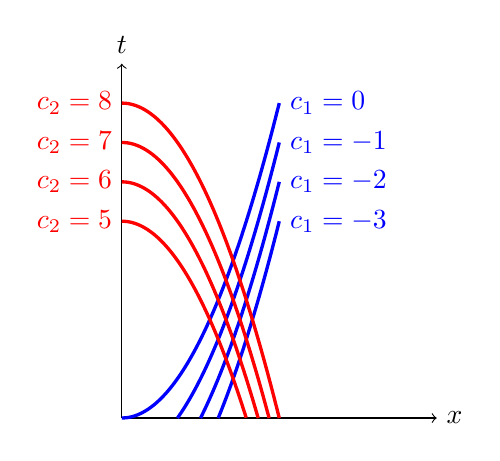
\begin{tikzpicture}
  \draw[->] (0,0) -- (4.,0) node[right] {$x$};
  \draw[->] (0,0) -- (0,4.5) node[above] {$t$};
  \draw[scale=0.5,domain=0:4,smooth,variable=\x,Blue,very thick] plot ({\x},{0.5*\x*\x}) node [right] {$c_1=0 $};
  \draw[scale=0.5,domain=1.4142:4,smooth,variable=\x,Blue,very thick] plot ({\x},{0.5*\x*\x-1}) node [right] {$c_1=-1$};
  \draw[scale=0.5,domain=2:4,smooth,variable=\x,Blue,very thick] plot ({\x},{0.5*\x*\x-2}) node [right] {$c_1=-2$};
  \draw[scale=0.5,domain=2.44948:4,smooth,variable=\x,Blue,very thick] plot ({\x},{0.5*\x*\x-3}) node [right] {$c_1=-3$};
  \draw[scale=0.5,domain=0:3.16,smooth,variable=\x,Red,very thick] plot ({\x},{-0.5*\x*\x+5});
  \node[left,Red] at (0,2.5) {$c_2=5$};
  \draw[scale=0.5,domain=0:3.4641,smooth,variable=\x,Red,very thick] plot ({\x},{-0.5*\x*\x+6});
  \node[left,Red] at (0,3) {$c_2=6$};
  \draw[scale=0.5,domain=0:3.7416,smooth,variable=\x,Red,very thick] plot ({\x},{-0.5*\x*\x+7});
  \node[left,Red] at (0,3.5) {$c_2=7$};
  \draw[scale=0.5,domain=0:4,smooth,variable=\x,Red,very thick] plot ({\x},{-0.5*\x*\x+8});
  \node[left,Red] at (0,4) {$c_2=8$};
\end{tikzpicture}
%%% Local Variables:
%%% mode: latex
%%% TeX-master: "../../mainManuscript"
%%% End:
}
  \subcaptionbox{Example \ref{ex:charac2}: $\lambda_{1}=1 \:\text{and} \: \lambda_2=1/2$\label{subfig:straight_lines}}{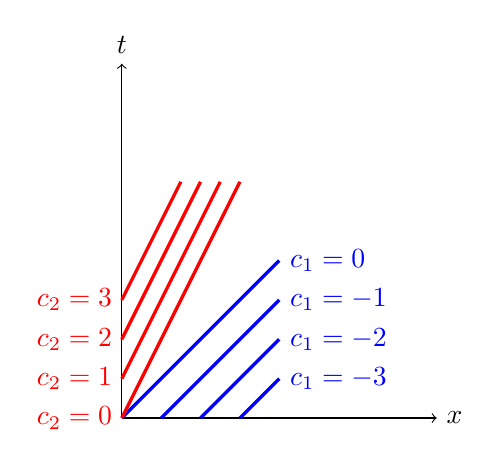
\begin{tikzpicture}
  \draw[->] (0,0) -- (4.,0) node[right] {$x$};
  \draw[->] (0,0) -- (0,4.5) node[above] {$t$};
  \draw[scale=0.5,domain=0:4,smooth,variable=\x,Blue,very thick] plot ({\x},{\x}) node [right] {$c_1=0$};
  \draw[scale=0.5,domain=1.:4,smooth,variable=\x,Blue,very thick] plot ({\x},{\x-1}) node [right] {$c_1=-1$};
  \draw[scale=0.5,domain=2:4,smooth,variable=\x,Blue,very thick] plot ({\x},{\x-2}) node [right] {$c_1=-2$};
  \draw[scale=0.5,domain=3:4,smooth,variable=\x,Blue,very thick] plot ({\x},{\x-3}) node [right] {$c_1=-3$};
  \draw[scale=0.5,domain=0:3,smooth,variable=\x,Red,very thick] plot ({\x},{2*\x});
  \node[left,Red] at (0,0) {$c_2=0$};
  \draw[scale=0.5,domain=-0.:2.5,smooth,variable=\x,Red,very thick] plot ({\x},{2*\x+1});
  \node[left,Red] at (0,0.5) {$c_2=1$};
  \draw[scale=0.5,domain=-0:2,smooth,variable=\x,Red,very thick] plot ({\x},{2*\x+2});
  \node[left,Red] at (0,1) {$c_2=2$};
  \draw[scale=0.5,domain=-0:1.5,smooth,variable=\x,Red,very thick] plot ({\x},{2*\x+3});
  \node[left,Red] at (0,1.5) {$c_2=3$};
\end{tikzpicture}
%%% Local Variables:
%%% mode: latex
%%% TeX-master: "../../mainManuscript"
%%% End:
}
  \caption{Family of base characteristic curves corresponding to the eigenvalues of the first order systems given in examples \ref{ex:charac1} and \ref{ex:charac2}.}
  \label{fig:exampleCharac}
\end{figure}

As theorem \ref{th:integral_surface_generated} states, an integral surface is generated by a one-parameter family of characteristic curves. Therefore the knowledge of those curves can be used to build the solution of the Cauchy problem. Indeed, the projection of the quasi-linear system \eqref{eq:1st_order_quasi-linear_syst} onto the \textit{left eigenbasis} or \textit{left characteristic basis} leads to:
\begin{equation*}
  \vect{\Lc}^k \( \Absf^t \vect{\Uc}_t + \Absf^x\vect{\Uc}_x \) + \vect{\Lc}^k \vect{\Sc}= \vect{0}
\end{equation*}
%Introduction of the definition of left eigenvectors \eqref{eq:eigenvectors} then yields:
where $\Lcb^k$ satisfies \eqref{eq:eigenvectors}, and hence:
\begin{equation*}
  \vect{\Lc}^k  \Absf^t \( \vect{\Uc}_t +\lambda_k \vect{\Uc}_x   \) + \vect{\Lc}^k \vect{\Sc}=\vect{0}
\end{equation*}
In this equation, the \textit{directional derivative} of $\vect{\Uc}$ along the $k$th characteristic curve arises, namely:
\begin{equation*}
 \ddroit{\Ucb}{t}\lvert_{t\in\varphi^k} = \Ucb_t + \lambda_k \Ucb_x   
\end{equation*}
Thus, along a characteristic curve a system of partial differential equations reduces to a system of \textit{Ordinary Differential Equations} (ODEs) composed of the following \textit{characteristic equations}:
\begin{equation}
  \label{eq:PDEs_ODEs}
  \vect{\Lc}^k  \Absf^t \(\ddroit{\Ucb}{t} + \Scb \)=\vect{0}
\end{equation}
Integration of equations \eqref{eq:PDEs_ODEs} yields a set of \textit{integral curves} from which the Cauchy problem can be solved.
%It then comes out that the Cauchy problem can be solved as the system \eqref{eq:PDEs_ODEs}.
Indeed, the solution at a point of the $(x,t)$ plane can be determined by tracing backward the characteristic curves to the initial curve and integrating ODEs \eqref{eq:PDEs_ODEs} along those paths according to the \textit{method of characteristics}. Note that if the right-hand side of equation \eqref{eq:1st_order_quasi-linear_syst} is zero, then $\Ucb$ is constant along characteristic curves. 

To illustrate the method, let us consider again the quasi-linear system of example \ref{ex:charac1} for which the Cauchy problem is built by prescribing initial conditions along the $x$-axis. Through a point $(x^*,t^*)$ pass two characteristic curves, each belonging to a different one-parameter family. The solution at this point can be determined by integrating the ODE corresponding to the first (\textit{resp. second}) eigenvalue of the system between $(x^1,0)$ (\textit{resp. $(x^2,0)$}) and $(x^*,t^*)$. The singularity of hyperbolic problems can hence be circumvented by using the characteristic structure in order to determine an unique solution. 
\begin{figure}[h]
  \centering
  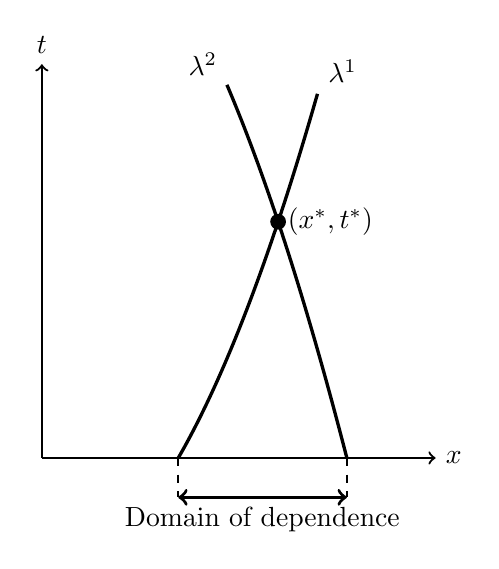
\begin{tikzpicture}
  \draw[thick,->](0,0)--(5,0) node [right] {$x$};
  \draw[thick,->](0,0)--(0,5) node [above] {$t$};
  % t1 = 0.5*x**2 + c1
  % t2 = -0.5*x**2 + c2
  % -> c1 = -1.5 ; c2 = 7.5
  % \draw[domain=1.7320508:3.5,smooth,variable=\x,Purple,very thick] plot ({\x},{0.5*\x*\x-1.5}) node [above right] {$t=\frac{x^2-3}{2}$};
  % \draw[domain=2.35:3.872983,smooth,variable=\x,Green,very thick] plot ({\x},{-0.5*\x*\x+7.5});
  \draw[domain=1.7320508:3.5,smooth,variable=\x,very thick] plot ({\x},{0.5*\x*\x-1.5}) node [above right] {$\lambda^1$};
  \draw[domain=2.35:3.872983,smooth,variable=\x,very thick] plot ({\x},{-0.5*\x*\x+7.5});
  % \node[left,Green] at (2.35,5) {$t=-\frac{x^2-15}{2}$};
  \node[left] at (2.35,5) {$\lambda^2$};
  \draw[<->,very thick] (1.7320508,-0.5) -- (3.872983,-0.5) ;
  \draw[dashed,thick] (1.7320508,0) -- (1.7320508,-0.5);
  \draw[dashed,thick] (3.872983,-0.) -- (3.872983,-0.5);
  \node[below] at (2.80,-0.5) {\text{Domain of dependence}};
  \fill[black] (3,3) circle (0.1) node [right] {$(x^*,t^*)$};
\end{tikzpicture}
%%% Local Variables:
%%% mode: latex
%%% TeX-master: "../../mainManuscript"
%%% End:

  \caption{Domain of dependence of the solution at point $(x^*,t^*)$ for the system of example \ref{ex:charac1}.}
  \label{fig:charac_method2x2}
\end{figure}
We see that only a segment of the initial curve has an influence on the solution at a given point. Namely, the intersections of the initial curve and characteristic curves with the highest and the lowest slopes define the \textit{domain of dependence} of the solution at this point (see figure \ref{fig:charac_method2x2}). This property of hyperbolic problems implies the existence of waves that propagates information at finite speeds corresponding to the eigenvalues of a quasi-linear form. The theory presented so far will be applied in what follows to solid mechanics.



%%% Local Variables:
%%% mode: latex
%%% TeX-master: "../mainManuscript"
%%% End:
